% \begin{figure}
%   \centering
%   \begin{tikzpicture}    
%     \node at (10, 0) {
%       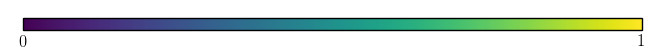
\includegraphics[height=4.2cm]{experiments/3d/vae_occ/easy_15/colorbar}
%     };
    
%     \node at (0, 0){
%       \includegraphics[width=6cm]{experiments/shapenet/vae_evae/easy_15/results_0}
%     };
    
%     \node at (6.5, 0){
%       \includegraphics[width=6cm]{experiments/shapenet/vae_evae/easy_15/results_3}
%     };
    
%     \draw[-,dashed](-3.5,-2.25) -- (10,-2.25);
    
%     % --- 
%     \node at (0, -4.5){
%       \includegraphics[width=6cm]{experiments/shapenet/vae_evae/moderate_15/results_0}
%     };
    
%     \node at (6.5, -4.5){
%       \includegraphics[width=6cm]{experiments/shapenet/vae_evae/moderate_15/results_3}
%     };
    
%     \draw[-,dashed](-3.5,-6.75) -- (10,-6.75);
    
%     % --- 
%     \node at (0, -9){
%       \includegraphics[width=6cm]{experiments/shapenet/vae_evae/hard_15_statistics/results_0}
%     };
    
%     \node at (6.5, -9){
%       \includegraphics[width=6cm]{experiments/shapenet/vae_evae/hard_15_statistics/results_3}
%     };
    

%     \node[rotate=90] at (-3.5, 0) {\easy};
%     \node[rotate=90] at (-3.5, -4.5) {\moderate};
%     \node[rotate=90] at (-3.5, -9) {\hard};
%     %\node at (3.25, 2.5) {reconstruction};
%   \end{tikzpicture}
%   \vskip 6px
  
%   \caption{Qualitative results for \EVAE on all three difficulties, \ie \easy,
%   \moderate and \hard. As before we present two samples for each difficulty,
%   showing the observed points, the partial free space, the target shape and
%   the predicted shape with its error. In all cases we show horizontal slices
%   of the corresponding volumes.}
%   \label{fig:appendix-experiments-shapenet-evae-qual}.
% \end{figure}
